\documentclass[12pt]{article}
\usepackage[utf8]{inputenc}
\usepackage[
	left=1.25in,
	right=1.25in,
	top=1in,
	bottom=1in]{geometry}
\usepackage{mathptmx}
\usepackage[dotinlabels]{titletoc}
\usepackage[nottoc,numbib]{tocbibind}
\usepackage[svgnames]{xcolor}
\usepackage{titlesec, setspace}
\usepackage{graphicx, caption}
\usepackage{hyperref, natbib}
% Journals
\newcommand{\aap}{A\&A}
\newcommand{\aj}{AJ}
\newcommand{\apj}{ApJ}
\newcommand{\araa}{ARA\&A}
\newcommand{\mnras}{MNRAS}
\newcommand{\nat}{Nature}
\newcommand{\pasa}{PASA}
\newcommand{\pasp}{PASP}
\newcommand{\physrep}{PhR}
\newcommand{\prd}{PhRvD}
\newcommand{\rpph}{RPPh}

% Page formatting
\geometry{
	left=1.25in,
	right=1.25in,
	top=1in,
	bottom=1in}
\hypersetup{
	colorlinks=true,
	citecolor=blue,
	filecolor=blue,
	linkcolor=blue,
	urlcolor=blue
}
\setlength{\footnotesep}{10pt}
\setlist{noitemsep}

% Fixing titlesec and hyperref interaction
\makeatletter
\def\ttl@useclass#1#2{%
\@ifstar
{\ttl@labeltrue\@dblarg{#1{#2}}}
{\ttl@labeltrue\@dblarg{#1{#2}}}}
\makeatother

% Image setup
\graphicspath{{figs/}}
\captionsetup[figure]{labelfont={bf}, font={small, stretch=1.3}, name={Figure}, labelsep=period}

% Section and subsection headings
\titleformat{\section}{\normalsize\bfseries\centering}{}{0em}{}
\titleformat{\subsection}{\normalsize\itshape\centering}{}{0.75em}{}
\newcommand{\nocontentsline}[3]{}
\newcommand{\tocless}[2]{\bgroup\let\addcontentsline=\nocontentsline#1{#2}\egroup}
\renewcommand{\contentsname}{Table of Contents}
\renewcommand{\abstractname}{{\normalsize\bfseries\centering{Abstract}}}
\renewcommand{\bibsection}{}

% For figures
\makeatletter
\setlength{\@fptop}{0pt plus 1fil}
\setlength{\@fpbot}{0pt plus 1fil}
\makeatother

% For formatting text and math
\let\vec\mathbf
\newcommand{\code}[1]{{\fontfamily{qcr}\selectfont#1}}
\newcommand{\red}[1]{\textcolor{red}{#1}}
\newcommand{\note}[1]{\textcolor{violet}{#1}}

% Special commands
\newcommand{\HI}{H\,\textsc{i}}
\newcommand{\OI}{O\,\textsc{i}}
\newcommand{\heraqm}{\code{hera\textunderscore qm}}
\newcommand{\herapspec}{\code{hera\textunderscore pspec}}
\newcommand{\herasim}{\code{hera\textunderscore sim}}
\newcommand{\pyuvdata}{\code{pyuvdata}}

\begin{document}
\doublespacing
\begin{center}
Environmental Systematics and the Impact on \\ 21-cm Epoch of Reionization Measurements \\
by \\
Lily R. Whitler \\
has been approved \\
Spring 2019 \vspace{0.1\textheight}

\begingroup
\renewcommand{\arraystretch}{0.7}
\begin{tabular}{p{1cm}p{3.5in}p{1cm}}
	& \centering APPROVED: & \\
	& & \\ & & \\
	& \hrulefill & \\
	& \hfill Prof. Daniel Jacobs, Director & \\
	& & \\ & & \\
	& \hrulefill & \\
	& \hfill Prof. Judd Bowman & \\
	& & \\ & & \\
	& \hrulefill & \\
	& \hfill Dr. Adam Beardsley &
\end{tabular} \vspace{0.075\textheight} \\
\begin{tabular}{p{1cm}p{3.5in}p{1cm}}
	& \centering ACCEPTED: & \\
	& & \\ & & \\
	& \hrulefill & \\
	& \hfill Dean, Barrett, The Honors College &
\end{tabular}
\endgroup
\end{center}
\thispagestyle{empty}
\newpage
\pagenumbering{arabic}

\begin{center}
	Environmental Systematics and the Impact on \\ 21-cm Epoch of Reionization Measurements \\
	by \\
	Lily R. Whitler
	
	\begin{spacing}{1}
		\vspace{0.15\textheight}
		A Thesis Presented in Partial Fulfillment \\
		of the Requirements for the Degree \\
		Bachelor of Science with Honors \\
		\vspace{0.22\textheight}
		Committee: \\
		Daniel Jacobs, Director \\
		Judd Bowman \\
		Adam Beardsley
	\end{spacing}

	\vspace{0.22\textheight}
	ARIZONA STATE UNIVERSITY \\
	April 2019
\end{center}
\thispagestyle{empty}
\newpage

\begingroup
\hypersetup{
	colorlinks=true,
	citecolor=DarkBlue,
	filecolor=black,
	linkcolor=black,
	urlcolor=DarkBlue
}
\tableofcontents
\listoffigures
\listoftables
\endgroup
\newpage

\begin{abstract}
\end{abstract}
\newpage

\section{Introduction} \label{sec:intro}

\subsection{The Epoch of Reionization} \label{subsec:eor}

Immediately after the Big Bang, the expanding universe was a hot, but cooling, plasma of fundamental particles. Approximately 380,000 years later, the universe had cooled and expanded enough for electrons to become bound to atomic nuclei, making the universe transparent to light and emitting the cosmic microwave background. Immediately following this period and lasting until $\sim$ 400 million years after the Big Bang was the cosmic Dark Ages, when the universe was quite literally dark---no stars or other sources of light had yet formed. Then, with the \red{formation} of the first luminous sources, the intergalactic medium (IGM), which had been predominantly neutral until then, was ionized by the energetic radiation from these sources during the Epoch or Reionization (EoR). The EoR ended around a billion years after the Big Bang, and the universe's structure has continued evolving into what we now see today. This history is summarized in Figure \ref{fig:timeline}. \red{I should probably have a reference here.}

\begin{figure}[tb]
	\centering
	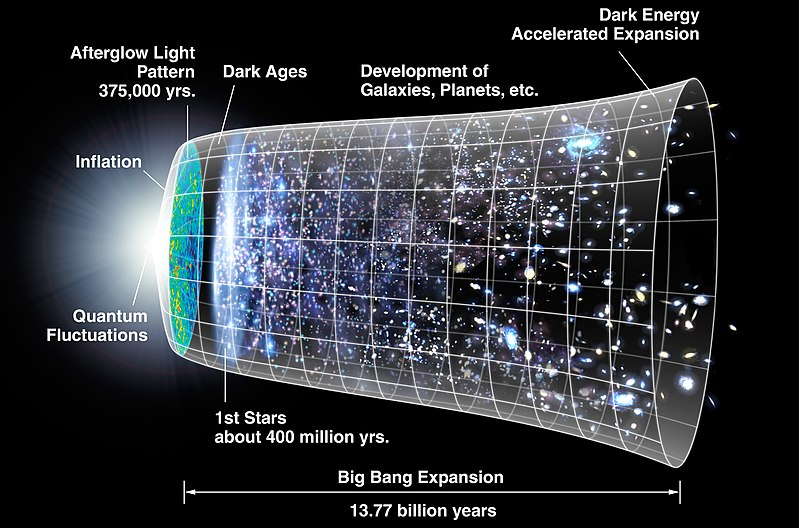
\includegraphics[width=\textwidth]{timeline.jpg}
	\caption[Timeline of the universe]{Timeline of the evolution of the universe. Image courtesy of NASA.}
	\label{fig:timeline}
\end{figure}

\cite{furlanetto2006}

\cite{morales2010}

\cite{pritchard2012}

\subsection{The 21-cm Power Spectrum} \label{subsec:ps}
\subsection{The Hydrogen Epoch of Reionization Array} \label{subsec:hera}
\begin{figure}[tb]
	\centering
	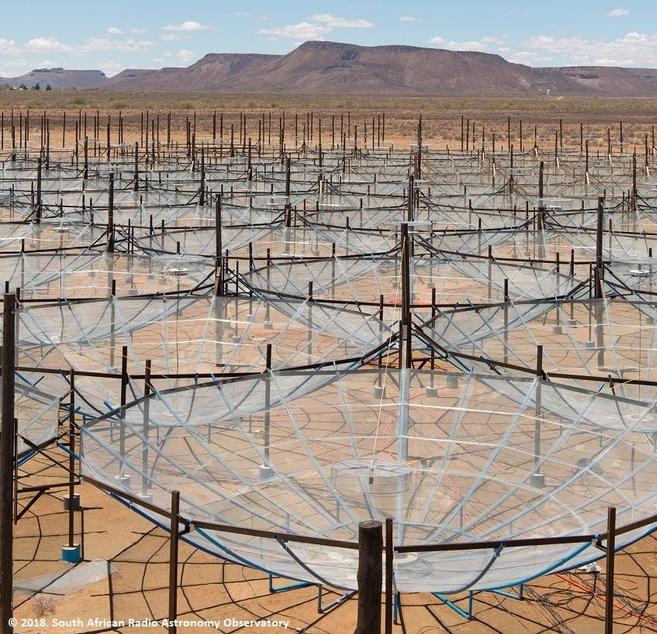
\includegraphics[width=0.75\textwidth]{hera.png}
	\caption[HERA as of late 2017 -- early 2018]{HERA as of late 2017 -- early 2018. HERA will observe large-scale structure prior to and during the EoR via the redshifted 21-cm line from the IGM. Image courtesy of the South African Radio Astronomy Observatory.}
	\label{fig:hera}
\end{figure}

The Hydrogen Epoch of Reionization Array (HERA; Figure \ref{fig:hera}) is an experiment to study the periods prior to and during the EoR \red{(from redshifts $z \sim 6 - 30$)} via measurements of the redshifted 21-cm line \citep{deboer2017}.
\subsection{Radio Frequency Interference} \label{subsec:rfi}

\section{Methods} \label{sec:methods}
\subsection{RFI Excision Strategies} \label{subsec:rfi_excision}
\subsection{Calculating the Power Spectrum} \label{subsec:calc_ps}
\subsection{Modelling HERA Data} \label{subsec:modelling}

\section{Results}

\section{Conclusion}

\bibliographystyle{apj}
\bibliography{refs}
\end{document}